%%%%%%%%%%%%%%%%%%%%%%%%%%%%%%%%%%%%%%%%%%%%%%%%%%%%%%%%%%%%%%%%%%%%%%%%%%%%%%%%%%
\begin{frame}[fragile]\frametitle{}
\begin{center}
{\Large Introduction to Swift for Tensorflow}
\end{center}
\end{frame}

%%%%%%%%%%%%%%%%%%%%%%%%%%%%%%%%%%%%%%%%%%%%%%%%%%%
\begin{frame}[fragile] \frametitle{Existing Approaches}

Existing approaches for building Neural Networks.

\begin{itemize}
\item Graph building: Pre-specific graph so that it can be made performant at run-time (TensorFlow 1.0) but hard to debug.
\item Eager Execution: Running tensor operations in interpreted code (TensorFlow 2.0), easy to debug, good usability, but bad on performance.
\end{itemize}

Need Usability + Performance.

\end{frame}

%%%%%%%%%%%%%%%%%%%%%%%%%%%%%%%%%%%%%%%%%%%%%%%%%%%
\begin{frame}[fragile] \frametitle{Usability + Performance}

\begin{itemize}
\item Need not just a new library
\item But a new language
\end{itemize}

That's Swift!!.

\end{frame}


%%%%%%%%%%%%%%%%%%%%%%%%%%%%%%%%%%%%%%%%%%%%%%%%%%%%%%%%%%%%%%%%%%%%%%%%%%%%%%%%%%%
\begin{frame}[fragile]\frametitle{Quote}
\begin{lstlisting}
"I always hope that when I start looking at a new language, there will be some mind-opening new ideas to find, and Swift definitely doesn't disappoint. Swift tries to be expressive, flexible, concise, safe, easy to use, and fast. Most languages compromise significantly in at least one of these areas."

- Jeremy Howard
\end{lstlisting}
\end{frame}

%%%%%%%%%%%%%%%%%%%%%%%%%%%%%%%%%%%%%%%%%%%%%%%%%%%%%%%%%%%%%%%%%%%%%%%%%%%%%%%%%%%
\begin{frame}[fragile]\frametitle{Quote}
\begin{lstlisting}
"PyTorch was created to overcome the gaps in Tensorflow. FastAI was built to fill gaps in tooling for PyTorch. But now we're hitting the limits of Python, and Swift has the potential to bridge this gap"

- Jeremy Howard
\end{lstlisting}
\end{frame}


%%%%%%%%%%%%%%%%%%%%%%%%%%%%%%%%%%%%%%%%%%%%%%%%%%%%%%%%%%%%%%%%%%%%%%%%%%%%%%%%%%%
\begin{frame} \frametitle{Swift Ecosystem}
\begin{center}
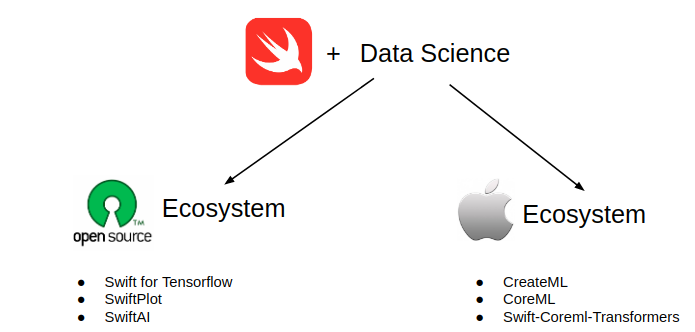
\includegraphics[width=0.9\linewidth,keepaspectratio]{s4tf2}
\end{center}

\begin{itemize}
\item Open-Source Swift runs on any machine.
\item For Apple ecosystem, need Apple machine to work on and you can only build for Apple devices like the iOS, macOS etc.
\end{itemize}

\end{frame}

%%%%%%%%%%%%%%%%%%%%%%%%%%%%%%%%%%%%%%%%%%%%%%%%%%%%%%%%%%%%%%%%%%%%%%%%%%%%%%%%%%%
\begin{frame} \frametitle{iOS/MacOS ML Apps}
\begin{center}
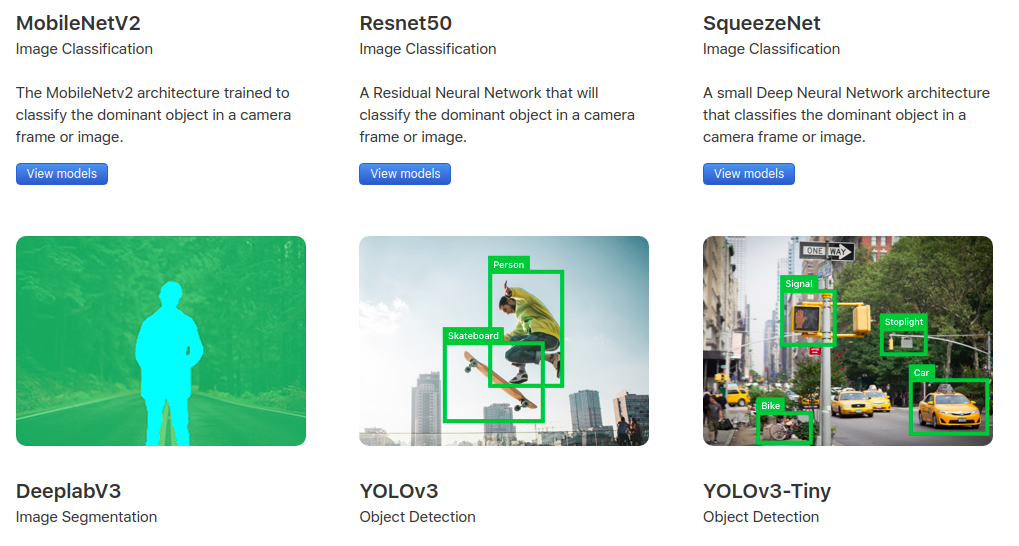
\includegraphics[width=0.9\linewidth,keepaspectratio]{s4tf3}
\end{center}
\end{frame}

%%%%%%%%%%%%%%%%%%%%%%%%%%%%%%%%%%%%%%%%%%%%%%%%%%%
\begin{frame}[fragile] \frametitle{How it all started?}

\begin{itemize}
\item In 2018, started as a small team in Google.
\item Swift is the first mainstream language with first-class language-integrated differentiable programming capabilities
\end{itemize}

\end{frame}

%%%%%%%%%%%%%%%%%%%%%%%%%%%%%%%%%%%%%%%%%%%%%%%%%%%%%%%%%%%%%%%%%%%%%%%%%%%%%%%%%%
\begin{frame}[fragile]\frametitle{}
\begin{center}
{\Large Why not Python?}
\end{center}
\end{frame}


%%%%%%%%%%%%%%%%%%%%%%%%%%%%%%%%%%%%%%%%%%%%%%%%%%%
\begin{frame}[fragile] \frametitle{Python, Today}

\begin{itemize}
\item Most used language in machine learning
\item Tons of library
\item So, why Swift? What’s wrong with Python?
\end{itemize}

\end{frame}

%%%%%%%%%%%%%%%%%%%%%%%%%%%%%%%%%%%%%%%%%%%%%%%%%%%
\begin{frame}[fragile] \frametitle{Why not Python?}

\begin{itemize}
\item To put it bluntly, Python is slow. 
\item Also, Python is not great for parallelism.
\item Python is usable, but inside its mostly \lstinline|C, C++|
\item External binaries:  limits developers to working on a small portion of the algorithm’s surface area. Cant debug in.
\item Library abstractions: you’ll have to use \lstinline|tf.print| and build a print node and not python \lstinline|print|
\end{itemize}

\end{frame}

%%%%%%%%%%%%%%%%%%%%%%%%%%%%%%%%%%%%%%%%%%%%%%%%%%%
\begin{frame}[fragile] \frametitle{Why Swift?}

\begin{itemize}
\item Swift allows you to program at a very high level, in an almost Pythonic way, while at the same time being really fast.
\item Fast, about 10x than Python.
\item No dynamic type changes. Strict at compile level.
\item Swift makes extensive use of closures (lambda functions),
\item In built differentiation, core to ML.
\item \lstinline|extension|, which allows us to add new functionality to any type, including the basic types.
\item Python interoperability
\item Finally, when you want to run production code, you can compile it and take advantage of the great optimization LLVM provides
\end{itemize}


{\tiny (Ref: Official details: https://docs.swift.org/swift-book/GuidedTour/GuidedTour.html)}

\end{frame}

%%%%%%%%%%%%%%%%%%%%%%%%%%%%%%%%%%%%%%%%%%%%%%%%%%%
\begin{frame}[fragile] \frametitle{Why Swift?}

All calls below are equivalent:

\begin{lstlisting}
let names = ["Chris", "Alex", "Ewa", "Barry", "Daniella"]
func backward(_ s1: String, _ s2: String) -> Bool {
    return s1 > s2
}
var reversedNames = names.sorted(by: backward)
reversedNames = names.sorted(by: { s1, s2 in return s1 > s2 } )
reversedNames = names.sorted(by: { s1, s2 in s1 > s2 } )
reversedNames = names.sorted(by: { $0 > $1 } )
reversedNames = names.sorted(by: >)
\end{lstlisting}

Making code extremely concise and readable.


\end{frame}

%%%%%%%%%%%%%%%%%%%%%%%%%%%%%%%%%%%%%%%%%%%%%%%%%%%%%%%%%%%%%%%%%%%%%%%%%%%%%%%%%%%
\begin{frame} \frametitle{What is Swift for Tensorflow?}
\begin{center}

\includegraphics[width=0.65\linewidth,keepaspectratio]{s4tf1}
\end{center}
\end{frame}

%%%%%%%%%%%%%%%%%%%%%%%%%%%%%%%%%%%%%%%%%%%%%%%%%%%
\begin{frame}[fragile] \frametitle{Swift for Tensorflow}

\begin{itemize}
\item Swift4Tensorflow isn’t just a Swift wrapper around TensorFlow but it’s being developed as a feature of the language itself. 
\item It is widely expected to become a core part of the language in the near future.
\item The library also adds many useful features to Swift like native support for automatic differentiation (which reminds me of Autograd in PyTorch) to make it even more compatible with numeric computing use-cases.
\end{itemize}

\begin{center}
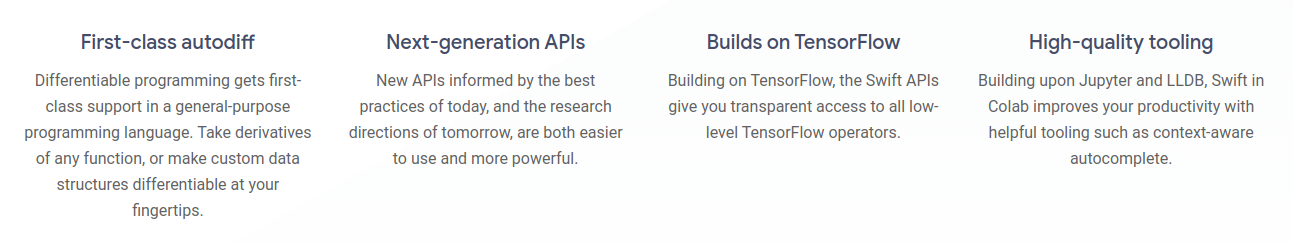
\includegraphics[width=\linewidth,keepaspectratio]{s4tf6}
\end{center}
\end{frame}

%%%%%%%%%%%%%%%%%%%%%%%%%%%%%%%%%%%%%%%%%%%%%%%%%%%
\begin{frame}[fragile] \frametitle{Swift for Tensorflow}

\begin{center}
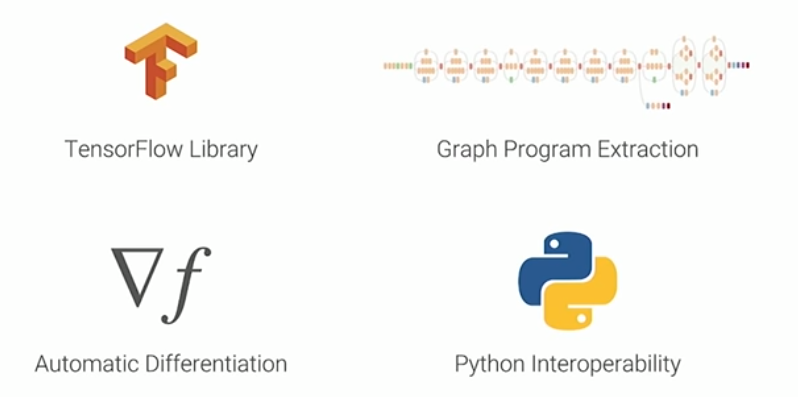
\includegraphics[width=\linewidth,keepaspectratio]{s4tf9}
\end{center}

{\tiny (Ref: Swift for TensorFlow (TensorFlow @ O’Reilly AI Conference, San Francisco '18) - Richard Wei)}
\end{frame}


%%%%%%%%%%%%%%%%%%%%%%%%%%%%%%%%%%%%%%%%%%%%%%%%%%%
\begin{frame}[fragile] \frametitle{Sample Neural Network}

\begin{center}
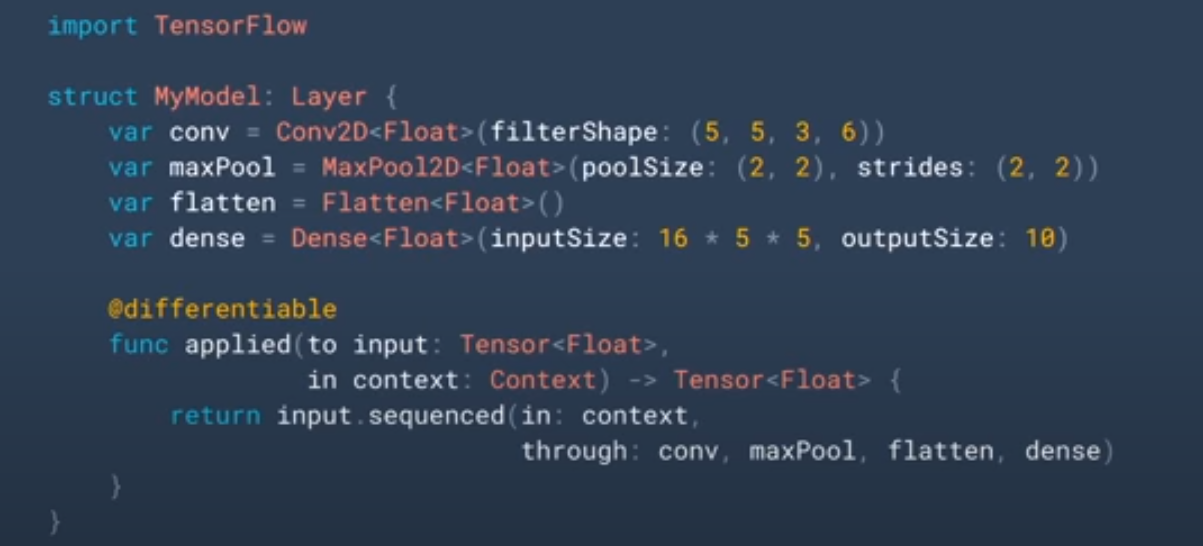
\includegraphics[width=0.65\linewidth,keepaspectratio]{s4tf7}

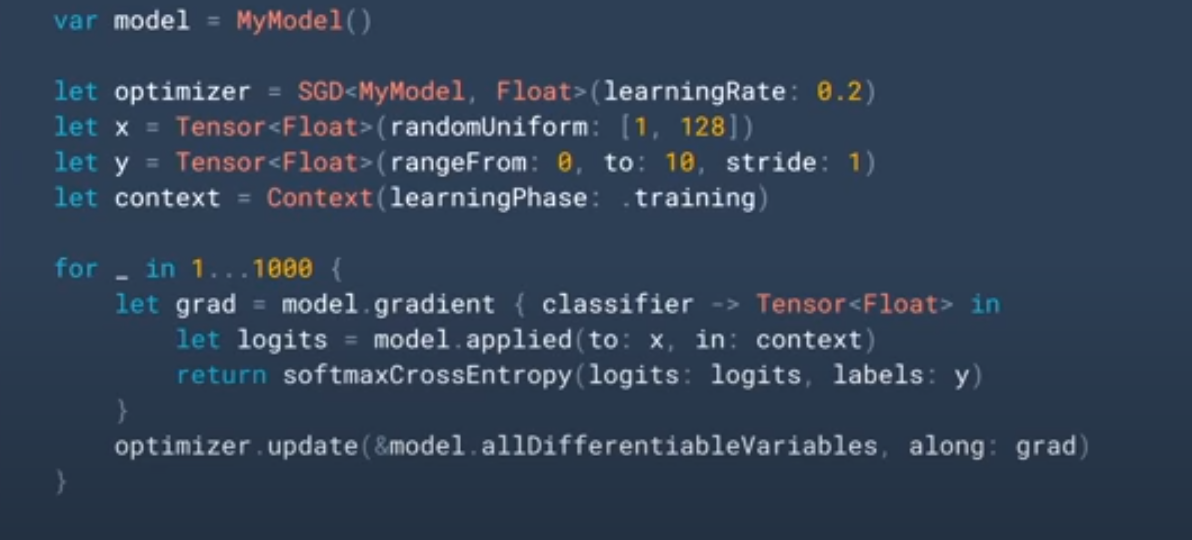
\includegraphics[width=0.65\linewidth,keepaspectratio]{s4tf8}
\end{center}

{\tiny (Ref: Swift for TensorFlow: The Next-Generation Machine Learning Framework (TF Dev Summit '19))}
\end{frame}

%%%%%%%%%%%%%%%%%%%%%%%%%%%%%%%%%%%%%%%%%%%%%%%%%%%
\begin{frame}[fragile] \frametitle{Graph Program Execution}

Why Swift For TensorFlow is fast even if its written like in Python like manner or like Eager execution way?

\begin{itemize}
\item The language itself is made fast.
\item Ifs, Loops, MatMul, Zip, etc Ops are identified and directly compiled into TensorFlow graphs, the binaries.
\item As its compiling the graph, it catches errors (such as shape errors or type errors) as well, before running.
\end{itemize}

\begin{center}
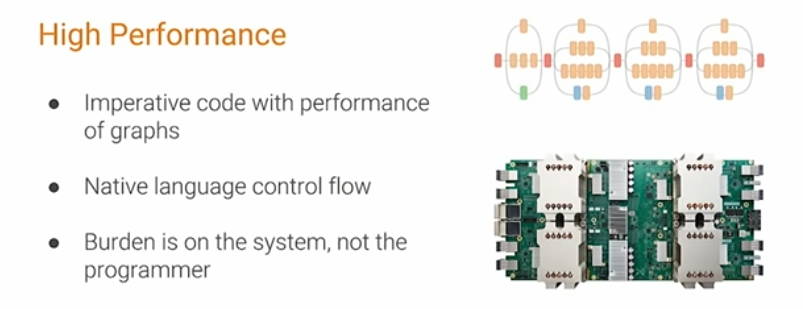
\includegraphics[width=0.65\linewidth,keepaspectratio]{s4tf10}
\end{center}
\end{frame}

%%%%%%%%%%%%%%%%%%%%%%%%%%%%%%%%%%%%%%%%%%%%%%%%%%%
\begin{frame}[fragile] \frametitle{Automatic Differentiation}

\begin{itemize}
\item AutoDiff (or AutoGrad in case of PyTorch) is generally implemented in library but for Swift its part of the language.
\item Works on standard library types, functions, etc. and also can make custom data structures, types differentiable as well.
\item \lstinline|gradient| is in built operator.
\item Using \lstinline|@differentiable| decorator for custom functions.
\item Compiler catches errors pointing to non-differentiable op.
\end{itemize}

\begin{center}
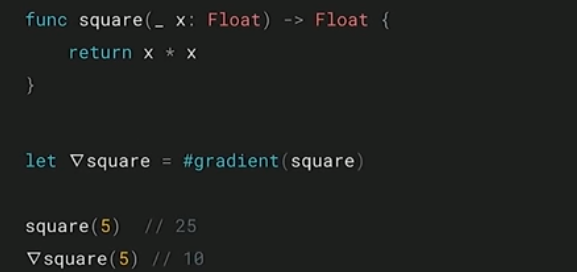
\includegraphics[width=0.65\linewidth,keepaspectratio]{s4tf11}
\end{center}
\end{frame}


%%%%%%%%%%%%%%%%%%%%%%%%%%%%%%%%%%%%%%%%%%%%%%%%%%%%%%%%%%%%%%%%%%%%%%%%%%%%%%%%%%
\begin{frame}[fragile]\frametitle{}
\begin{center}
{\Large What Next \ldots }
\end{center}
\end{frame}


%%%%%%%%%%%%%%%%%%%%%%%%%%%%%%%%%%%%%%%%%%%%%%%%%%%
\begin{frame}[fragile] \frametitle{Future of Swift for Tensorflow}

\begin{itemize}
\item Currently, it is in infancy and the libraries around data science and numeric computing are still developing.
\item Has a strong industry backing behind it.
\item Swift will have a rich ecosystem of tools and libraries- maybe even better than what Python has today.
\end{itemize}

\end{frame}
